\chapter{2022年\textsf{HDU}「普通物理1」期中试题解答}

\begin{minipage}{0.32\textwidth}
    \textbf{开课学院}：理学院
      
    \textbf{课程编码}：A0715011s
\end{minipage}
\hfill
\begin{minipage}{0.32\textwidth}
    \textbf{解析制作}：\textsc{Mingyu Hsia}

    \textbf{\,\hologo{TeX}~排版}：\textsc{Mingyu Hsia}
\end{minipage}
\hfill
\begin{minipage}{0.15\textwidth}
    \centering
    \begin{tikzpicture}
        \node [inner sep=0] at (0,0) {
            \qrcode[height=3em,version=4]{https://qm.qq.com/q/Jd5GTWrMAs}};
        \fill [color=white,rounded corners=(sqrt(2)+2)/11*1em] (-.5em,-.5em) rectangle (.5em,.5em);
        \node [inner sep=0] at (0,0) {\color{MidnightBlue}\scriptsize\faIcon{qq}};
    \end{tikzpicture}

    \scriptsize\href{https://qm.qq.com/q/Jd5GTWrMAs}{\itshape 未央物理营\! $^\dagger$}
\end{minipage}
\hfill
\begin{minipage}{0.15\textwidth}
    \centering
    \begin{tikzpicture}
        \node [inner sep=0] at (0,0) {
            \qrcode[height=3em,version=4]{http://weixin.qq.com/r/DBIABcHEqgnWKIVmb0eI}};
            \fill [color=white,rounded corners=(sqrt(2)+2)/11*1em] (-.5em,-.5em) rectangle (.5em,.5em);
        \node [inner sep=0] at (0,0) {\color{DarkGreen}\scriptsize\faIcon{weixin}};
    \end{tikzpicture}

    \scriptsize\href{http://weixin.qq.com/r/DBIABcHEqgnWKIVmb0eI}{\itshape 未央学社}
\end{minipage}

\section{选择题（每题3分，共27分）}

\begin{problem} % {平均速度与平均速率}
质点沿半径为$R$的圆周做匀速率运动，每$T$秒转一圈. 在$2T$时间间隔中其平均速度大小与平均速率大小分别为
\begin{tasks}(4)
    \task $2\pi R/T$，$2\pi R/T$
    \task $0$，$0$
    \task[\true] $0$，$2\pi R/T$
    \task $2\pi R/T$，$0$
\end{tasks}
\end{problem}
\begin{solution}
    位移$\Delta \bm x=0$，路程$s=2\times 2\pi R$. 所以$\abs{\overline{\bm v}}=\abs{\Delta\bm x/\Delta t}=0$，$\overline{v}=\Delta s/\Delta t=2\pi R/T$.
\end{solution}

\begin{problem}
    已知水星的半径是地球半径的$0.4$倍，质量为地球的$0.04$倍. 设在地球上的重力加速度为$g$，则水星表面上的重力加速度为
\begin{tasks}(4)
\task[\true] $0.25g$
\task $0.1g$
\task $2.5g$
\task $4g$
\end{tasks}
\end{problem}
\solute2
\begin{solution}
    由引力提供重力$GMm/R^2=mg$得$g=GM/R^2\propto M/R^2$. 由于水星的半径是地球半径的$0.4$倍，质量为地球的$0.04$倍，所以其表面上的重力加速度为$g'=0.04/0.4^2\times g=0.25g$.
\end{solution}

\begin{paracol}{2}
\begin{problem}
    有一接地的金属球，用一弹簧吊起，金属球原来不带电. 若在它的下方放置一电荷为$q$的点电荷，则
    \begin{tasks}(2)
    \task 只有$q>0$金属球才下移
    \task 只有$q<0$金属球才下移
    \task 无论$q$正负金属球都不动
    \task[\true] 无论$q$正负金属球都下移
    \end{tasks}
    \switchcolumn\vspace*{\fill}\centering
    \begin{circuitikz}[scale=.8]
        \wall{(-1,0)}{(1,0.2)};
        \draw [very thick,decoration={aspect=0.6, segment length=10, amplitude=5,coil},decorate] (0,0) -- (0,-2.1); %amplitude调整螺线管的直径，segment length调整间距
        \shade [ball color=blue!60!red!80!gray!10] (0,-2.3) circle (0.2);
        \draw (0,-2) -- (1,-2) -- (1,-2.5) node [ground] {};
        \filldraw (0,-2.7) circle (0.05);
        \node [right] at (0,-2.7) {$q$};
    \end{circuitikz}\vspace*{\fill}
\end{problem}
\end{paracol}
\begin{solution}
    无论$q$带正电还是负电，其都会使金属球下表面产生与其电性相反的感应电荷，所以二者始终存在吸引力，金属球就会下移.
\end{solution}

\begin{paracol}{2}
    \begin{problem}
        如图所示，在点电荷$+q$电场中，若取图中$P$点处为电势零点，则$M$点的电势为
        \begin{tasks}(4)
            \task[\true] $-q/8\pi\epsilon_0a$
            \task $q/8\pi\epsilon_0a$
            \task $-q/4\pi\epsilon_0a$
            \task $q/4\pi\epsilon_0a$
        \end{tasks}
    \end{problem}
    \switchcolumn\vspace*{\fill}\centering
    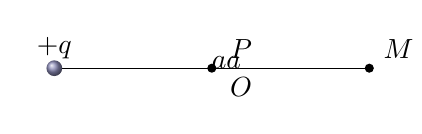
\begin{tikzpicture}
        \draw (-2,0) -- (2,0);
        \shade [ball color=MidnightBlue!50] (-2,0) circle (.1);
        \node [above] at (-2,0) {$+q$};
        \filldraw (0,0) circle (.05);
        \filldraw (2,0) circle (.05);
        \length{(-2,-1)}{(0,-1)}{$a$}{(.5,0)};
        \length{(0,-1)}{(2,-1)}{$a$}{(.5,0)};
        \node [below] at (0,0) {$O$};
        \node [above] at (0,0) {$P$};
        \node [above] at (2,0) {$M$};
    \end{tikzpicture}\vspace*{\fill}
\end{paracol}
\solute3
\begin{solution}\leavevmode
    \begin{itemize}
        \item 正常情况下，$P$点、$M$点的电势分别为$\varphi_P=q/4\pi\epsilon_0a$，$\varphi_M=q/8\pi\epsilon_0a$.
        \item 取图中$P$点为电势零点，图中所有点的电势都要减去$P$点原来的电势，此时$\varphi_P'=0$.
        \item 所以$M$点的电势为$\varphi_M'=\varphi_M-\varphi_P=-q/8\pi\epsilon_0a$.
    \end{itemize}
\end{solution}

\begin{problem}
有两个半径相同，质量相等的细圆环$A$和$B$.$A$环的质量分布均匀，$B$环的质量分布不均匀.它们对通过环心并与环面垂直的轴的转动惯量分别为$I_A$和$I_B$，则
\begin{tasks}(5)
\task $I_A>I_B$
\task $I_A<I_B$
\task[\true] $I_A=I_B$
\task* 不能确定$I_A$、$I_B$哪个大
\end{tasks}
\end{problem}
\begin{solution}
    由于圆环上各点与环心处转轴的距离相同，则$r_i^2$项可从转动惯量求和式中提取出来，最终其转动惯量只与圆环的总质量有关，与质量分布无关，即$I=\sum{m_ir_i^2}=R^2\sum{m_i}=MR^2$.
\end{solution}

\begin{paracol}{2}
\begin{problem}
    质量为$m$的小球，放在光滑的木板和光滑的墙壁之间，并保持平衡，如图所示.设木板和墙壁之间的夹角为$\alpha$，当$\alpha$逐渐增大时，小球对木板的压力将
    \begin{tasks}(6)
        \task 增加
        \task 不变
        \task[\true] 减小
        \task* 先增后减，分界角为$45^{\circ}$
    \end{tasks}
\switchcolumn\vspace*{\fill}\centering
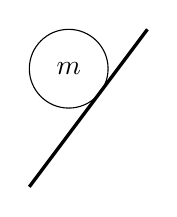
\begin{tikzpicture}[scale=.5]
    \draw [very thick] (0,0) -- (3,4);
    \begin{scope}[rotate=90]
        \wall{(-.2,0)}{(4.2,.2)};
    \end{scope}
    \draw (1,3) circle (1) node {$m$};
\end{tikzpicture}\vspace*{\fill}
\end{problem}
\end{paracol}
\begin{solution}
    小球对木板的压力$N=mg/\sin\alpha$，所以$\alpha$增大，小球对木板的压力减小.
\end{solution}

\begin{problem}
    关于刚体对轴的转动惯量，下列说法中正确的是
    \begin{tasks}
        \task 只取决于刚体的质量，与质量的空间分布和轴的位置无关
        \task 取决于刚体的质量和质量的空间分布，与轴的位置无关
        \task 只取决于转轴的位置，与刚体的质量和质量的空间分布无关
        \task[\true] 取决于刚体的质量、质量的空间分布和轴的位置
    \end{tasks}
\end{problem}

\begin{paracol}{2}
\begin{problem}
    真空中有一点电荷$Q$，在与它相距为$r$的$a$点处有一实验电荷$q$.现使$q$从$a$点沿半圆轨道运动到$b$点，如图所示.则电场力对$q$做功为
    \begin{tasks}(7)
        \task*(2) $\displaystyle\frac{Qq}{4\pi\epsilon_0 r^2}\cdot\frac{\pi r^2}{2}$
        \task*(2) $\displaystyle\frac{Qq}{4\pi\epsilon_0 r^2}\cdot 2r$
        \task[\true] $0$
        \task*(2) $\displaystyle\frac{Qq}{4\pi\epsilon_0 r^2}\cdot\pi r$
    \end{tasks}
    \switchcolumn\vspace*{\fill}\centering
    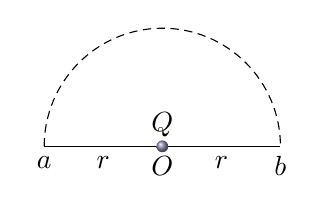
\begin{tikzpicture}[scale=1.5]
        \draw (-1,0) node [below] {$a$} -- (1,0) node [near start,below] {$r$} node [midway,below] {$O$} node [midway,above] {$Q$} node [near end,below] {$r$} node [below] {$b$};
        \draw [densely dashed] (-1,0) arc (180:0:1);
        \shade [ball color=MidnightBlue!50] (0,0) circle (.05);
    \end{tikzpicture}\vspace*{\fill}
\end{problem}
\end{paracol}
\begin{solution}
    $q$从$a$点到$b$点，二者与$Q$的距离相同，所以$q$的电势能不变，电场力对$q$做功为零.
\end{solution}

\begin{problem}{B}
已知一高斯面所包围的体积内电量代数和$\sum{q_i}=0$，则可肯定
\begin{tasks}(2)
\task 高斯面上各点场强均为零
\task 穿过整个高斯面的电通量为零
\task 穿过高斯面上每一面元的电通量均为零
\task 以上说法都对
\end{tasks}
\end{problem}
\begin{solution}
    高斯面所包围的体积内电量代数和为零，只能说明高斯面所包围的体积内电量代数和为零，但并不代表穿过高斯面上每一面元的电通量均为零，因为高斯面上各点场强方向可指向高斯面外，也可指向高斯面内，所以A、C选项错误.
\end{solution}

\section{填空题（每题3分，共21分）}

\begin{problem}
一质点作半径为$\qty{0.1}\m$的圆周运动，其角位置的运动学方程为$\theta=\frac{\pi}{4}+\frac{1}{2}t^2$，则其切向加速度为$a_t=$\ans{$\qty{0.1}{\m/\s^2}$}.
\end{problem}
\begin{solution}
角加速度$\ddot\theta=\qty1{\radian\cdot\s^{-2}}$，切向加速度$a_\tau=R\beta=\qty{0.1}{\m/\s^2}$.
\end{solution}

\begin{problem}
    有一人造地球卫星，质量为$m$，在地球表面上空$3$倍于地球半径$R$的高度沿圆轨道运行，用$m$、$R$、引力常数$G$和地球质量$M$表示，则卫星的动能为\ans{$GMm/8R$}.
\end{problem}
\begin{solution}
    由引力提供向心力$GMm/(4R)^2=mv^2/4R$得卫星的动能$E_k=mv^2/2=GMm/8R$.
\end{solution}

\begin{problem}
    质量为$m$的质点以速度$\bm v$沿一直线运动，则它对直线外垂直距离为$l$的一点的角动量大小是\ans{$mvl$}.
\end{problem}

\begin{paracol}{2}
\begin{problem} % {高斯定理}
    一均匀带电直导线长为$L$，电荷线密度为$+\gamma$.过导线中点$O$作一半径为$R$（$R>L/2$）的球面$S$，$P$为带电直导线的延长线与球面$S$的交点.则通过该球面的电场强度通量$\Phi_e=$\ans{$\gamma L/\epsilon_0$}.
    \switchcolumn\vspace*{\fill}\centering
    \begin{tikzpicture}[scale=.6]
        \draw (0,0) circle (2);
        \draw [->] (-2,0) node [left] {$P$} -- (0,0) node [above] {$O$} -- (1,{sqrt(3)}) node [above right] {$R$};
        \filldraw (-2,0) circle (.05);
        \filldraw [pattern=north east lines] (-.8,-.1) -- (-.8,.1) -- (.8,.1) -- (.8,-.1)--cycle;
        \length{(-.8,-.5)}{(.8,-.5)}{$L$}{(.5,0)};
    \end{tikzpicture}\vspace*{\fill}
\end{problem}
\switchcolumn
\begin{solution}
    由高斯定理得$\Phi_e=\gamma L/\epsilon_0$.
\end{solution}
\end{paracol}

\begin{problem}
    两同心导体球壳，内球壳带电荷$+q$，外球壳带电荷$-2q$.静电平衡时，外球壳的电荷分布为：内表面\ans{$-q$}，外表面\ans{$-q$}.
\end{problem}
\begin{solution}
    内球壳会在外球壳内表面产生$-q$的感应电荷，外表面产生$+q$的感应电荷. 叠加上外球壳外表面原有的电荷量$-2q$后得外球壳外表面带电量为$-q$.
\end{solution}

\begin{paracol}{2}
    \begin{problem}
        质量分别为$m$和$2m$的两物体（都可视为质点），用一长为$l$的轻质刚性细杆相连，系统绕通过杆且垂直的竖直固定轴$O$转动，已知$O$轴离质量为$2m$的质点的距离为$l/3$，质量为$m$的质点的线速度为$v$且与杆垂直，则该系统对转轴的角动量大小\ans{$mvl$}.
        \switchcolumn\vspace*{\fill}\centering
        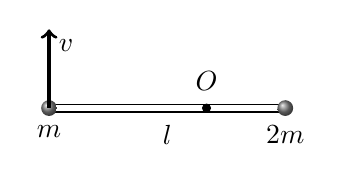
\begin{tikzpicture}
            \draw (0,-.05) -- (3,-.05) -- (3,.05) -- (0,.05)--cycle;
            \shade [ball color=gray] (0,0) circle (.1);
            \shade [ball color=gray] (3,0) circle (.1);
            \draw [very thick,->] (0,0) -- (0,1);
            \node [right] at (0,.8) {$v$};
            \filldraw (2,0) circle (.05);
            \node [below] at (0,-.1) {$m$};
            \node [below] at (1.5,-.1) {$l$};
            \node [below] at (3,-.1) {$2m$};
            \node [above] at (2,.1) {$O$};
        \end{tikzpicture}\vspace*{\fill}
    \end{problem}
\end{paracol}
\solute4\solute*{为节约资源，本试题计算题部分不提供演算区域，请自备稿纸，或在下页边缘书写.}
\begin{solution}
    系统角速度$\displaystyle\omega=v/(2l/3)=3v/2l$，角动量$L=I\omega=[m\cdot(2l/3)^2+2m\cdot(l/3)^2]\omega=mvl$.
\end{solution}

\begin{paracol}{2}
\begin{problem}
    在点电荷$+q$与$-q$的静电场中，作出如图所示的三个闭合曲面$S_1$、$S_2$、$S_3$，则通过这些闭合面的电场强度通量分别是：\ans{$\Phi_1=q/\epsilon_0$，$\Phi_2=0$，$\Phi_3=-q/\epsilon_0$}.
    \switchcolumn\vspace*{\fill}\centering
    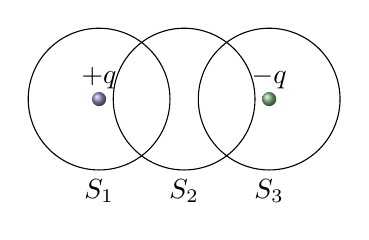
\begin{tikzpicture}[scale=.9]
        \shade [ball color=MidnightBlue!50] (-1.2,0) circle (.1);
        \shade [ball color=DarkGreen!50] (1.2,0) circle (.1);
        \draw (0,0) circle (1);
        \draw (-1.2,0) circle (1);
        \draw (1.2,0) circle (1);
        \node [above] at (-1.2,0) {$+q$};
        \node [above] at (1.2,0) {$-q$};
        \node [below] at (-1.2,-1) {$S_1$};
        \node [below] at (0,-1) {$S_2$};
        \node [below] at (1.2,-1) {$S_3$};
    \end{tikzpicture}\vspace*{\fill}
\end{problem}\switchcolumn
\solute2
\begin{solution}
    $S_1$内有电荷$q$，$S_2$内没有电荷，$S_3$内有电荷$-q$. 由高斯定理得三个闭合曲面的电通量分别为$q/\epsilon_0$，$0$，$-q/\epsilon_0$.
\end{solution}
\end{paracol}

\clearpage

\section{计算题（共52分）}

\begin{problem}
    一个弹簧下端挂质量为$\qty{0.1}\kg$的砝码时长度为$\qty{0.07}\m$，挂$\qty{0.2}\kg$的砝码时长度为$\qty{0.09}\m$.现在把此弹簧放在光滑桌面上，并要沿水平方向从长度$l_1=\qty{0.10}\m$缓慢拉长到$l_2=\qty{0.14}\m$，外力需做功多少？
\end{problem}
\begin{solution}\leavevmode
    \begin{itemize}
        \item 弹簧的劲度系数$k=(F_2-F_1)/(x_2-x_1)=(0.2-0.1)g/(0.09-0.07)=\qty{50}{\N\cdot\m^{-1}}$.
        \item 弹簧原长$l_0=0.07-0.1g/50=\qty{0.05}\m$.
        \item 外力做功$W=\int_{l_1-l_0}^{l_2-l_0}{kx\d x}=\frac{1}{2}kx^2\big|_{l_1-l_0}^{l_2-l_0}=\qty{0.14}\J$.
    \end{itemize}
\end{solution}

\begin{problem}
    质量为$\qty5\kg$的一水桶悬于绕在辘轳上的轻绳下端，辘轳可视为一质量为$\qty{10}\kg$的圆柱体.桶从井口由静止释放，求桶下落过程中绳中的张力. 辘轳绕轴转动时的转动惯量为$MR^2/2$，其中$M$和$R$分别为辘轳的质量和半径，轴上摩擦忽略不计.
\end{problem}
\begin{solution}
    设绳中张力为$T$. 分别对桶列牛顿运动定律、对辘轳列转动定律得
    \[\begin{cases}
        mg-T=ma\\
        TR=\frac{1}{2}MR^2\beta
    \end{cases}\]
    代入关系$a=R\beta$得桶下落过程中绳中的张力$T=Mmg/(M+2m)$.
\end{solution}

\begin{problem}
    两个无限长同轴柱圆柱面，半径分别为$R_1$，$R_2$（$R_2>R_1$）带有等值异号电荷，每单位长度的电量为$\lambda$，试求
    \begin{tasks}[label=\arabic*.](2)
        \task $r>R_2$时离轴线为$r$处的电场强度.
        \task $R_1<r<R_2$时离轴线为$r$处的电场强度.
    \end{tasks}
\end{problem}
\solute1
\begin{solution}\leavevmode
    \begin{enumerate}
        \item 取半径$r>R_2$，高度为$l$的圆柱高斯面，由高斯定理$E_1\cdot 2\pi rl=[+\lambda l+\ab(-\lambda)l]/\epsilon_0$得$E_1=0$.
        \item 取半径$R_1<r<R_2$，高度为$l$的圆柱高斯面，由高斯定理$E_2\cdot 2\pi rl=\lambda l/\epsilon_0$得$E_2=\lambda/2\pi r\epsilon_0$.
    \end{enumerate}
\end{solution}

\begin{paracol}{2}
\begin{problem}
    如图：$AB=2L$，$OCD$是以$B$为中心，$L$为半径的半圆，$A,\ B$处分别有正负电荷$+q,\ -q$.试问：把单位正电荷从$O$沿$OCD$移动到$D$，电场力对它做了多少功？
    \switchcolumn\centering
    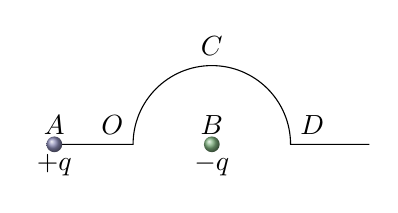
\begin{tikzpicture}
        \draw (-2,0) node [above] {$A$} node [below] {$+q$} -- (-1,0) node [above left] {$O$} arc (180:0:1) node [above,midway] {$C$} node [above right] {$D$} -- (2,0);
        \shade [ball color=MidnightBlue!50] (-2,0) circle (0.1);
        \shade [ball color=DarkGreen!50] (0,0) circle (0.1) node [above] {$B$} node [below] {$-q$};
    \end{tikzpicture}
\end{problem}
\end{paracol}
\begin{solution}
    由于电场力是保守力，单位正电荷移动前后与$-q$的距离相等，$-q$产生的电场对其不做功. 以$A$为原点，水平向右为$x$轴方向. $+q$产生的电场分布为$E=q/4\pi\epsilon_0 x^2$，电场力做功为
    \[W=\int_L^{3L}{q_0E\d x}=\frac{qq_0}{4\pi\epsilon_0}\int_L^{3L}{\frac{1}{x^2}}=\frac{qq_0}{4\pi\epsilon_0}\frac{2}{3L}\xlongequal[q_0=1]{\text{单位电荷}}\frac{1}{6\pi\epsilon_0L}\]
\end{solution}

\begin{problem}
一质点沿$x$轴运动，其加速度为$a=6t$ (SI).已知当$t=0$时，质点位于$x_0=\qty5\m$处，初速度$v_0=0$.试求其位移和时间的关系式.
\end{problem}
\begin{solution}\leavevmode
    \begin{itemize}
        \item 质点的速度表达式$v=\int{a\d t}\xlongequal{t=0,v=0}3t^2$.
        \item 质点的位移表达式$x=\int{v\d t}\xlongequal{t=0,x=5}t^3+5$.
    \end{itemize}
\end{solution}

\begin{paracol}{2}
\begin{problem}
    一半径为$R_1$的球体均匀带正电，体电荷密度为$\rho$，球内有一半径为$R_2$的小球形空腔，空腔中心$O'$与球心$O$相距为$a$，如图所示.
    \begin{enumerate}
        \item 求空腔内$P$点处的电场强度$\bm E$.
        \item 画出空腔内电力线的分布.
        \item 求空腔中心$O'$处的电势.
    \end{enumerate}
    \switchcolumn\vspace*{\fill}\centering
    \begin{tikzpicture}[scale=.85]
        \draw (0,0) circle (2) node [below right] {$O$};
        \draw ({sqrt(3)-1},{sqrt(3)-1}) circle (.5);
        \fill (0,0) circle (.05);
        \fill ({sqrt(2)/2},{sqrt(2)/2}) circle (.05) node [below] {$O'$};
        \node at (1,1) {$*$};
        \draw [densely dashed] (0,0) circle ({sqrt(2)});
    
        \filldraw [pattern color=MidnightBlue,pattern=north east lines,thick] ({sqrt(3)-1},{sqrt(3)-1}) circle (0.5);
        \draw [very thick,dashed,->] (-.5,-.5) -- (2,2);
    \end{tikzpicture}\vspace*{\fill}
\end{problem}
\end{paracol}
\begin{solution}\leavevmode
    \begin{enumerate}
        \item $P$点场强由体电荷密度为$+\rho$的球体和$O'$处体电荷密度为$-\rho$的球体两部分组成.
        \begin{itemize}
            \item 对于电荷密度为$+\rho$的球体，由于均匀带电球壳内部场强为零，所以只有$r<OP$部分的球体对这部分场强有贡献. 由高斯定理$E_1\cdot 4\pi OP^2=\frac43\rho\pi OP^3/\epsilon_0$得此部分在$P$点场强为$\bm E_1=\rho\cdot\bm{OP}/3\epsilon_0$.
            \item 对于电荷密度为$-\rho$的球体，同理可知只有$r<O'P$部分的球体对这部分场强有贡献. 由高斯定理得$\bm E_2=-\rho\cdot\bm{O'P}/3\epsilon_0$.
            \item 综上所述，$P$点场强为$\bm E=\bm E_1+\bm E_2=\rho\bm{OO'}/3\epsilon_0=\rho a\widehat{\bm{OO'}}/3\epsilon_0$.
        \end{itemize}
        \addtocounter{enumi}{1}
        \item $O'$处电势由以下三部分组成.
        \begin{itemize}
            \item $r<OO'$部分带电球体在$O'$的电势可看作等电量点电荷在$O'$的电势，即
            \[\varphi_\text{ia}=\frac{1}{4\pi\epsilon_0}\frac{\rho\cdot\frac{4}{3}\pi a^3}{a}=\frac{\rho a^2}{3\epsilon_0}\]
            \item $r>OO'$部分带电厚球壳在$O'$的电势可看作无数个薄球壳的电势累加，即
            \[\varphi_\text{ib}=\int_a^{R_1}{\frac{1}{4\pi\epsilon_0}\frac{\rho\cdot 4\pi r^2\d r}{r}}=\frac{\rho(R_1^2-a^2)}{2\epsilon_0}\]
            \item 对于电荷密度为$-\rho$的球体，只需将上方积分下限变为$0$即可$\varphi_\text{ii}=-\rho R_2^2/2\epsilon_0$.
            \item 综上所述，$O'$点电势为$\varphi=\varphi_\text{ia}+\varphi_\text{ib}+\varphi_\text{ii}=\rho(3R_1^2-3R_2^2-a^2)/6\epsilon_0$.
        \end{itemize}
    \end{enumerate}
\end{solution}

\begin{paracol}{2}
\begin{problem}
    如图所示，质量为$m_2$的物体与轻弹簧相连，弹簧另一端与一个质量可忽略的挡板连接，静止在光滑的桌面上. 弹簧劲度系数为$k$. 今有一质量为$m_1$，速度为$\bm v_0$的物体向弹簧运动并与挡板正碰，求弹簧最大的被压缩量.
    \switchcolumn\vspace*{\fill}\centering
    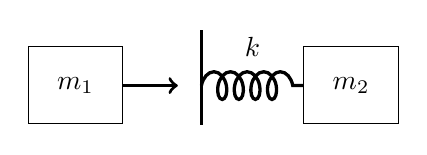
\begin{tikzpicture}
        \wall{(-2.5,0)}{(2.5,-.2)};
        \draw (-2.2,.02) rectangle (-1,1);
        \draw [very thick,->] (-1,.5) -- (-.3,.5);
        \draw [very thick] (0,0) -- (0,1.2);
        \draw (1.3,.02) rectangle (2.5,1);
        \draw [very thick,decoration={aspect=.6, segment length=6, amplitude=5,coil},decorate] (0,.5) -- (1.3,.5); %amplitude调整螺线管的直径，segment length调整间距
        \node at (-1.6,.5) {$m_1$};
        \node at (1.9,.5) {$m_2$};
        \node [above] at (.65,.75) {$k$};
    \end{tikzpicture}\vspace*{\fill}
\end{problem}
\end{paracol}
\begin{solution}
    刚碰撞后$m_1$的速度大于$m_2$，弹簧不断压缩. 当$m_1$和$m_2$共速时，弹簧压缩量最大，弹性势能最大. 物块、弹簧、挡板组成的系统在水平方向上动量守恒和系统机械能守恒可分别列出
    \[\begin{cases}
        m_1v_0=(m_1+m_2)v\\
        \frac12mv_0^2=\frac12(m_1+m_2)v^2+E_p
    \end{cases}\]
    联立得弹簧的最大弹性势能为$E_p=m_1m_2v_0^2/2(m_1+m_2)$. 根据弹簧弹性势能表达式$E_p=k\Delta x^2/2$得弹簧的最大压缩量$\Delta x_{\max}=v_0\sqrt{m_1m_2/k(m_1+m_2)}$.
\end{solution}

\begin{paracol}{2}
\begin{problem}
    一半径为$R$、转动惯量为$I$的圆柱体$B$，可绕水平固定的中心轴$O$无摩擦地转动. 起初圆柱体静止，一质量为$M$的木块以速度$v_1$在光滑水平面上向右滑动，并擦过圆柱体的上表面跃上另一同高度的光滑表面，如图. 设它和圆柱体脱离接触前，它们之间无相对滑动. 试求木块的最后速率$v_2$.
    \switchcolumn\vspace*{\fill}\centering
    \begin{tikzpicture}[scale=.75]
        \draw [very thick,line cap=butt] (-2.8,0) -- (-.8,0) -- (-.8,-1.8);
        \fill [pattern=north east lines] (-2.8,0) rectangle (-.8,-.3) rectangle (-1.1,-1.8);
        \draw [very thick] (2.8,0) -- (.8,0) -- (.8,-1.8);
        \fill [pattern=north east lines] (2.8,0) rectangle (.8,-.3) rectangle (1.1,-1.8);
        \draw (0,-.5) circle (.5) node [left] {$\scriptscriptstyle O$} node [above] {$\scriptscriptstyle B$} -- (0,-1);
        \fill (0,-.5) circle (.05);
        \draw (-1.3,0) rectangle (-2,.5) node [midway] {$\scriptstyle M$};
        \draw [very thick,->] (-1.9,.75) -- (-1.4,.75) node [near end,above] {$\scriptstyle\bm v_1$};
        \draw [dashed] (1.3,0) rectangle (2,.5);
        \draw [very thick,->] (1.4,.75) -- (1.9,.75) node [near end,above] {$\scriptstyle\bm v_2$};
    \end{tikzpicture}
\end{problem}
\end{paracol}
\begin{solution}
    由物块和圆筒对$O$点角动量守恒得$mv_1R=mv_2R+I\omega$. 擦过圆柱体的过程中，二者之间无相对滑动，代入纯滚动约束$v=\omega R$得$v_2=mv_1R^2/(I+mR^2)$.
\end{solution}